% Chapter Template

\chapter{Ensayos y resultados} % Main chapter title

\label{Chapter4} % Change X to a consecutive number; for referencing this chapter elsewhere, use \ref{ChapterX}

En este capítulo se describen las pruebas realizadas para validar el hardware y el firmware desarrollados. Con el objetivo de verificar la precisión y robustez del sistema, se utilizaron herramientas de automatización de pruebas y hardware externo que permitieron contrastar y analizar los datos capturados por cada sensor. Estas pruebas revelaron el rendimiento del sistema y evaluaron el cumplimiento de los requisitos establecidos por cada módulo.

%----------------------------------------------------------------------------------------
%	SECTION 1
%----------------------------------------------------------------------------------------

\section{Pruebas unitarias del firmware}
\label{sec:pruebas_unitarias}

En esta sección se presentan pruebas unitarias para validar las funcionalidades clave del software, lo que asegura la precisión y estabilidad de cada componente. Durante la implementación de los drivers, se aplicó la metodología de desarrollo Test-Driven Development (TDD) \citep{ieee2023}, que establece la creación de pruebas unitarias antes de cada módulo y garantiza que el código cumpla con los requerimientos especificados desde las primeras etapas. Esta metodología permitió identificar errores y realizar ajustes con anticipación, optimizando la calidad del software. Para el desarrollo de pruebas automáticas, se empleó Ceedling, una herramienta robusta que facilitó la creación, ejecución y gestión de pruebas, asegurando una verificación consistente de cada funcionalidad.

\subsection{Prueba del sensor DHT11}
Para validar la implementación del driver del sensor DHT11, se emplearon informes de cobertura generados por Ceedling. Esta metodología no solo verificó la correcta adquisición de datos de temperatura y humedad, sino que también permitió evaluar la cobertura de las pruebas.

El reporte del código fue fundamental para identificar áreas del driver que no estaban cubiertas por las pruebas iniciales, lo que permitió realizar ajustes y optimizaciones en el código para asegurar una validación exhaustiva. Además, los resúmenes de resultados generados en consola ofrecieron una vista rápida y clara del desempeño de las pruebas.

\newpage

La cobertura obtenida mediante estas pruebas unitarias aseguró que el firmware estuviera preparado para manejar situaciones como valores atípicos o desconexiones inesperadas del sensor. Así, el proceso de validación del driver del DHT11 proporcionó no solo datos sobre el rendimiento y la cobertura del código, sino que también contribuyó a mejorar la confiabilidad y precisión del sistema en su conjunto. En la figura \ref{fig:test_sensor_dht11} se presentan los resultados de la prueba realizada.

\vspace{1cm}

\begin{figure}[htbp]
	\centering
	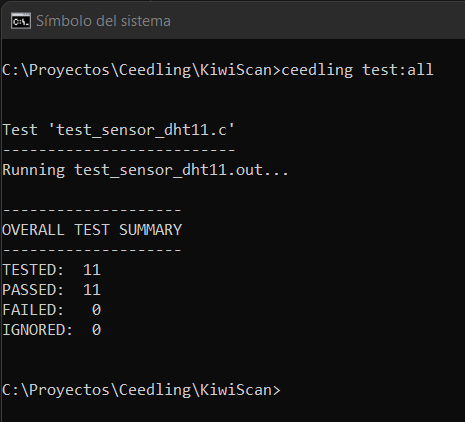
\includegraphics[width=0.7\textwidth, height=0.3\textheight]{./Figures/test_sensor_dht11.png}
	\caption{Test realizado al driver DHT11.}
	\label{fig:test_sensor_dht11}
\end{figure}

\vspace{1cm}

\subsection{Prueba del display LCD}

El driver del display LCD cumplió con múltiples requisitos, incluyendo la visualización de datos en tiempo real, cantidad de capturas tomadas, distancia del objetivo y alertas generadas, sin afectar el desempeño general del sistema. Ceedling proporcionó un resumen detallado de las métricas de prueba, que reflejó la cantidad de casos exitosos y fallidos, así como la cobertura de cada función en el driver.

Las pruebas revelaron detalles específicos sobre la interacción con el hardware, como la capacidad de la pantalla para responder a comandos de refresco rápido. En particular, los informes de cobertura destacaron áreas del driver con potencial de optimización, como la gestión de excepciones ante fallos de comunicación con el display. Esta observación motivó mejoras en la codificación del driver, fortaleciendo la detección y manejo de errores y, con ello, asegurando que el display muestre la información correcta.

Además, se validaron las capacidades del driver para recibir y mostrar correctamente la información generada por otros módulos, como los datos de los sensores de temperatura y humedad, el lector de tarjetas SD y el de distancia. Los resultados se presentan en la figura \ref{fig:test_lcd_display}.

\vspace{1cm}

\begin{figure}[htbp]
	\centering
	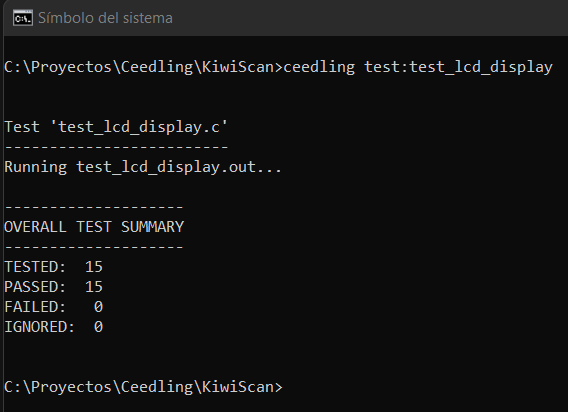
\includegraphics[width=0.7\textwidth, height=0.3\textheight]{./Figures/test_lcd_display.png}
	\caption{Test realizado al display LCD.}
	\label{fig:test_lcd_display}
\end{figure}

\vspace{1cm}

\subsection{Prueba de cámara Ov7670}

La validación del driver de la cámara Ov7670 fue fundamental para garantizar que el sistema capturara imágenes con precisión y fiabilidad, cumpliendo los requisitos en términos de resolución y capacidad de captura en tiempo real.

La prueba incluyó aspectos clave, como la inicialización de la cámara, la captura de imágenes en diferentes resoluciones y la transmisión de datos al proceso principal para su almacenamiento y análisis.

Durante las pruebas, se evaluaron distintas configuraciones de la cámara Ov7670, verificando los ajustes de resolución y formato de imagen. La cobertura obtenida en las pruebas reflejó la capacidad del driver para mantener la estabilidad y calidad en la captura de imágenes incluso en condiciones de carga intensa. Además, los informes de prueba permitieron identificar y solucionar fallas menores, como errores en la sincronización del módulo de captura o posibles pérdidas de datos en resoluciones altas, asegurando un flujo constante y sin interrupciones. La figura \ref{fig:test_ov7670_camera}
muestra los resultados de las pruebas realizadas.

Otro aspecto evaluado fue la integración del driver con el sistema general, garantizando que las imágenes capturadas por la cámara se transfirieran correctamente a los módulos de procesamiento y almacenamiento sin afectar el rendimiento del firmware. Este proceso resultó crucial para validar la robustez del sistema ante interrupciones inesperadas, verificando que el driver de la cámara mantuviera estabilidad y asegurará la disponibilidad de imágenes para el procesamiento posterior.

\vspace{1cm}

\begin{figure}[htbp]
	\centering
	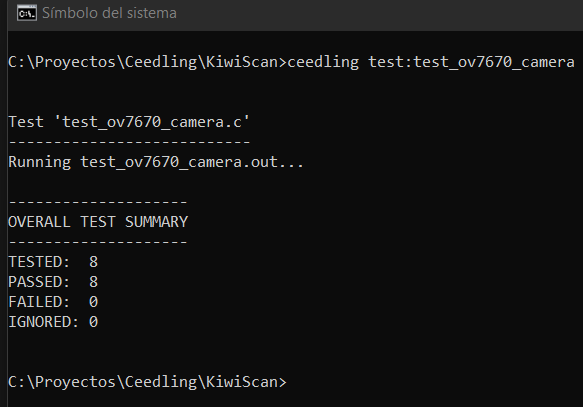
\includegraphics[width=0.7\textwidth, height=0.3\textheight]{./Figures/test_ov7670_camera.png}
	\caption{Test realizado a la cámara Ov7670.}
	\label{fig:test_ov7670_camera}
\end{figure}

\vspace{1cm}

\subsection{Prueba del sensor ultrasónico HC-SR04}

El proceso de prueba abarcó varias funciones clave del driver, incluyendo la inicialización del sensor, el envío de pulsos de activación, y la recepción y procesamiento de los ecos de respuesta que miden la distancia. Ceedling ejecutó pruebas unitarias para cada una de estas funciones, generando informes detallados sobre la precisión y consistencia de los resultados. Este enfoque garantizó que el sensor ofreciera mediciones confiables y respondiera adecuadamente ante diferentes distancias, desde rangos cortos hasta los límites efectivos del sensor.

Otra área de prueba clave fue la integración del sensor con el sistema general y la manera en que el driver del HC-SR04 gestionaba las interrupciones durante la medición de distancias. Esta verificación fue esencial para confirmar que el sistema mantuviera un flujo de datos continuo, entregando información precisa en tiempo real al módulo de procesamiento.

Finalmente, se realizaron pruebas para analizar el manejo de errores en el driver, especialmente en situaciones en las que el sensor no recibía respuesta de eco o detectaba obstrucciones inesperadas. Se validó que el sistema reaccionara correctamente ante estas situaciones, registrando la falta de datos o enviando alertas al proceso de alarmas cuando fuera necesario. La figura \ref{fig:test_hc_sr04_sensor} muestra los resultados de las pruebas realizadas.

\newpage

\vspace{1cm}

\begin{figure}[htbp]
	\centering
	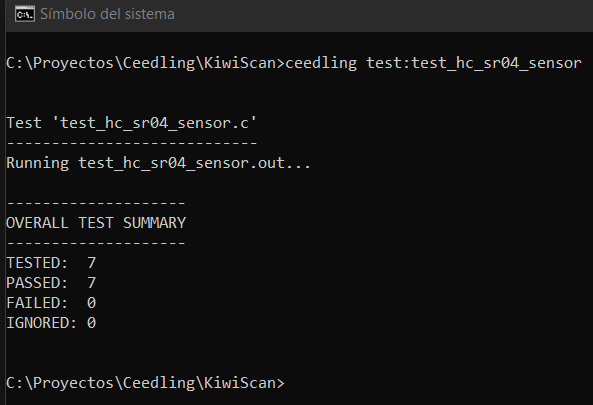
\includegraphics[width=0.7\textwidth, height=0.3\textheight]{./Figures/test_hc_sr04_sensor.png}
	\caption{Test realizado al sensor ultrasónico HC-SR04.}
	\label{fig:test_hc_sr04_sensor}
\end{figure}

\vspace{1cm}

\subsection{Prueba del lector de tarjetas SD}

Las pruebas iniciales evaluaron las operaciones de escritura y lectura, funciones esenciales para el almacenamiento continuo de datos capturados por los sensores. Cada operación fue probada con diferentes tamaños de archivos, simulando diversos escenarios de uso, desde pequeñas cantidades de datos hasta archivos de mayor tamaño, para determinar la capacidad del driver para manejar un flujo de datos sostenido.

Otro aspecto clave de las pruebas fue la verificación de la funcionalidad de borrado y la gestión del espacio disponible en la tarjeta SD. Se comprobó que el driver eliminaba datos de forma efectiva y detectaba con la cantidad de espacio liberado y restante tras cada operación.

Además, se evaluaron las capacidades del driver para detectar y gestionar tarjetas SD con diferentes formatos. La lectura y escritura en tarjetas formateadas en sistemas FAT32 y exFAT permitió verificar la flexibilidad del driver y su compatibilidad con distintos tipos de almacenamiento. Este aspecto fue crítico, pues garantiza que el sistema se adapte a diversas tarjetas sin requerir reconfiguraciones manuales.

Se simularon problemas comunes, como la extracción inesperada de la tarjeta, errores en la escritura y fallos de inicialización. Esto permitió observar cómo el driver respondía ante estos fallos, verificando que el sistema registrará la interrupción o emitiera alertas adecuadas sin comprometer la estabilidad del sistema. La figura \ref{fig:test_sd_card_reader} muestra los resultados de las pruebas realizadas.

\vspace{1cm}

\begin{figure}[htbp]
	\centering
	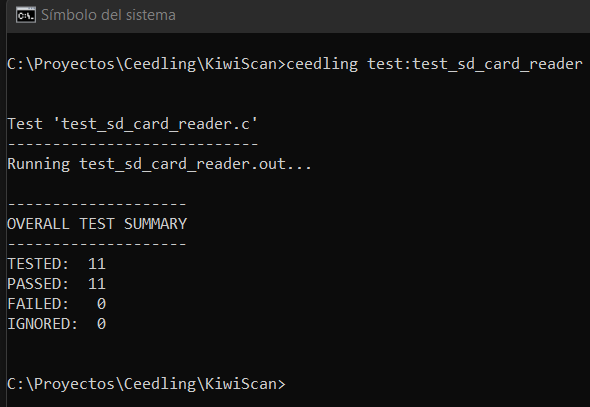
\includegraphics[width=0.7\textwidth, height=0.3\textheight]{./Figures/test_sd_card_reader.png}
	\caption{Test realizado al lector de tarjetas SD.}
	\label{fig:test_sd_card_reader}
\end{figure}

\vspace{1cm}

\subsection{Prueba de integración de drivers}

La prueba de integración de drivers tuvo como objetivo evaluar el desempeño conjunto de los componentes desarrollados y comprobar su funcionamiento de manera coordinada y sin interferencias. Esta prueba incluyó los drivers del sensor de temperatura y humedad DHT11, el sensor ultrasónico HC-SR04, la cámara OV7670, el display LCD y el lector de tarjetas SD, los cuales operaron simultáneamente para asegurar una respuesta del sistema.

En el proceso, cada driver fue evaluado en condiciones similares a las de su operación final, verificando la capacidad del sistema para gestionar la entrada y salida de datos sin fallas, interferencias ni retrasos perceptibles en los tiempos de respuesta. Los resultados indicaron que todos los drivers se integraron correctamente, funcionando sin dificultades en los ensayos realizados, con una sincronización adecuada entre los distintos módulos. La figura \ref{fig:test_integrated_drivers} muestra los resultados obtenidos.

Las pruebas confirmaron que el sistema responde adecuadamente a las demandas de funcionamiento en conjunto, sin comprometer la velocidad ni la precisión de las mediciones y salidas visuales.

\newpage

\vspace{1cm}

\begin{figure}[htbp]
	\centering
	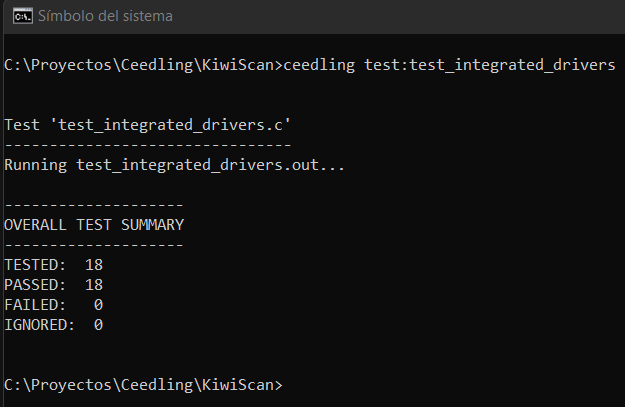
\includegraphics[width=0.7\textwidth, height=0.3\textheight]{./Figures/test_integrated_drivers.png}
	\caption{Test de integración de drivers.}
	\label{fig:test_integrated_drivers}
\end{figure}

\vspace{1cm}

\section{Pruebas funcionales del hardware}
\label{pruebas_funcionales_hardware}

Esta sección expone los ensayos realizados para evaluar la precisión y confiabilidad de los sensores integrados en el sistema. El propósito principal es contrastar las mediciones del sensor de temperatura y humedad DHT11, el sensor ultrasónico HC-SR04 y la cámara Ov7670 con las obtenidas por otros dispositivos o herramientas.

\subsection{Evaluación de precisión en temperatura y humedad del sensor DHT11}

Para determinar la precisión del sensor DHT11 en la medición de temperatura y humedad, se realizaron pruebas comparativas utilizando un termómetro higrómetro de laboratorio como referencia. Esta prueba tuvo lugar durante un periodo de dos horas, con mediciones cada 15 minutos a partir del mediodía. La prueba se llevó a cabo en un entorno controlado, con una temperatura base aproximada de 25 ° C, en horario de verano.

En cada intervalo de tiempo, se registraron los datos de temperatura y humedad captados por ambos dispositivos, lo que permitió identificar las diferencias entre el sensor DHT11 y el termómetro higrómetro. Se observó que el DHT11 reportó variaciones de entre 1 y 2 puntos respecto a la referencia de laboratorio, tanto en temperatura como en humedad, lo que muestra una desviación mínima. Los resultados de esta comparación se presentan en la tabla \ref{tab:DHT11_comparacion}.

\newpage

\begin{table}[h]
    \centering
    \caption[Comparación de mediciones de temperatura y humedad]{Comparación de mediciones de temperatura y humedad.}
    \begin{tabularx}{\textwidth}{l X X X X X X X}  % Cambia el ancho de la última columna
        \toprule
        \textbf{Hora} & \textbf{Temp. DHT11} & \textbf{Temp. higrómetro} & \textbf{Dif. temp.} & \textbf{Hum. DHT11} & \textbf{Hum. higrómetro} & \textbf{Dif. hum.} \\
        \midrule
        12:00 PM & 25.5 & 25.0 & +0.5 & 47 & 49 & -2\\		
        12:15 PM & 26.0 & 25.5 & +0.5 & 46 & 48	& -2\\
        12:30 PM & 26.3 & 26.0 & +0.3 & 48 & 49 & -1\\
        12:45 PM & 26.5 & 26.2 & +0.3 & 49 & 50 & -1\\
        01:00 PM & 26.7 & 26.5 & +0.2 & 50 & 52 & -2\\
        01:15 PM & 27.0 & 26.8 & +0.2 & 51 & 53 & -2\\
        01:30 PM & 27.2 & 27.0 & +0.2 & 52 & 54 & -2\\
        01:45 PM & 27.3 & 27.1 & +0.2 & 52 & 54 & -2\\
        02:00 PM & 27.5 & 27.3 & +0.2 & 53 & 55 & -2\\
        \bottomrule
    \end{tabularx}
    \label{tab:DHT11_comparacion}
\end{table}

\subsection{Análisis de precisión en medición de distancia con el sensor ultrasónico HC-SR04}

El objetivo de esta prueba fue evaluar la precisión del sensor ultrasónico HC-SR04 en la medición de distancias. Se establecieron seis puntos de referencia a distintas distancias de una muestra de una planta de kiwi: 50 centímetros, 1 metro, 1.5 metros, 2 metros, 2.5 metros y 3 metros. Las mediciones de referencia se obtuvieron con una cinta métrica convencional, y luego se registraron las lecturas del sensor HC-SR04 para cada posición.

Los resultados evidencian que el sensor HC-SR04 presenta una gran precisión en distancias cortas, detectando sin errores la medida de 50 centímetros. Sin embargo, conforme aumenta la distancia, se observan diferencias leves que van de 1 a 5 centímetros en comparación con la referencia. Estos datos demuestran que el sensor es bastante preciso en rangos de hasta un metro y mantiene una tolerancia aceptable para aplicaciones de detección de distancias mayores. La tabla \ref{tab:HCSR04_comparacion} resume las mediciones obtenidas.

\newpage

\begin{table}[h]
	\centering
	\caption[Comparación de mediciones tomadas]{Comparación de mediciones tomadas.}
	\begin{tabular}{c c c}    
		\toprule
		\textbf{Distancia de referencia (cm)} 	 & \textbf{Medición del HC-SR04 (cm)} 		& \textbf{Diferencia (cm)}  \\
		\midrule
		50 & 50 & 0 \\		
		100 & 101 & +1 \\	
		150 & 151 & +1 \\	
            200 & 202 & +2 \\	
            250 & 253 & +3 \\	
            300 & 305 & +5 \\	
		\bottomrule
		\hline
	\end{tabular}
	\label{tab:HCSR04_comparacion}
\end{table}

\subsection{Evaluación de calidad en la captura de imágenes con la cámara Ov7670}

La evaluación de la calidad de imagen de la cámara OV7670 se realizó mediante la comparación de capturas obtenidas con una cámara fotográfica digital Samsung WB550. Ambos dispositivos capturaron imágenes de una planta de kiwi como objetivo principal. Esta prueba se centró en analizar la capacidad de la OV7670 para reproducir detalles y colores en tres resoluciones compatibles: 640x480, 800x600 y 1024x768. Todas las imágenes se almacenaron en formato JPEG, lo que garantizó que el formato de archivo fuera el mismo en ambas cámaras para una comparación uniforme.

Los resultados reflejan una calidad de captura buena en el módulo OV7670, logrando una representación fiel de la planta en términos de detalles generales. Sin embargo, en cuanto a la intensidad de color y la nitidez, las imágenes capturadas por la Samsung WB550 muestran una mayor saturación de colores y una precisión más alta en la definición de detalles finos. La Samsung WB550, al ser un dispositivo diseñado para la fotografía, exhibe capacidades superiores en la reproducción cromática y en la claridad de los contornos, elementos fundamentales para la evaluación de imágenes de calidad.

La comparación entre ambas cámaras demostró que, aunque la OV7670 es adecuada para aplicaciones de captura básica y cumplió con los requisitos del proyecto, la Samsung WB550 mantiene una ventaja significativa en la calidad visual. En la figura \ref{fig:comparacion_fotos} se presenta una comparación visual entre ambas cámaras en una resolución de 800x600, mostrando claramente las diferencias en la calidad de imagen.

\newpage

\begin{figure}[!htpb]
     \centering
     \begin{subfigure}[b]{1.0\textwidth}
         \centering
         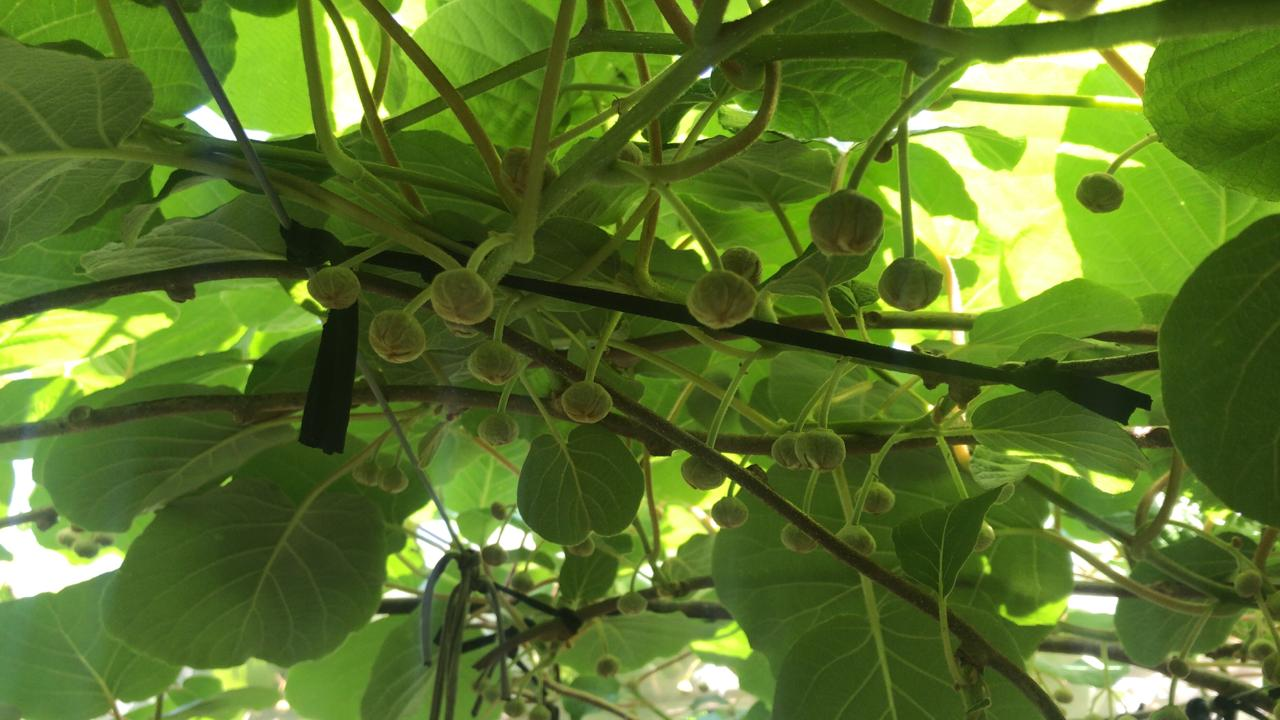
\includegraphics[width=.80\textwidth]{./Figures/kiwi_samsung.jpg}
         \caption{Foto con cámara Samsung Wb550.}
         \label{fig:1de2}
     \end{subfigure}
     \hfill
     \begin{subfigure}[b]{1.0\textwidth}
         \centering
         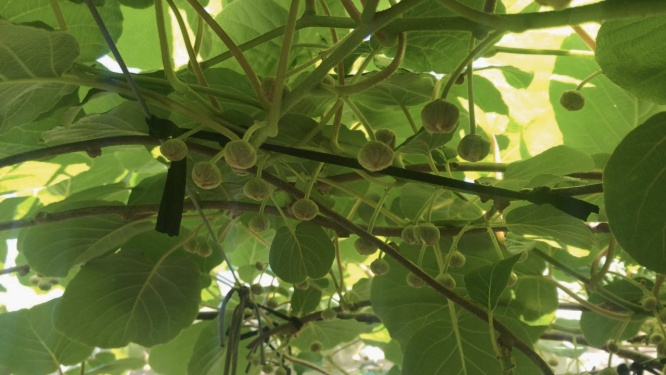
\includegraphics[width=.80\textwidth]{./Figures/kiwi_Ov7670.jpg}
         \caption{Foto con cámara Ov7670.}
         \label{fig:2de2}
     \end{subfigure}
     \hfill

        \caption{Comparación de capturas realizadas.}
        \label{fig:comparacion_fotos}
\end{figure}

\section{Pruebas de campo}
\label{pruebas_de_campo}

La realización de pruebas de campo constituye una etapa fundamental en la validación de sistemas destinados a operar en entornos reales. Sin embargo, en el contexto de este proyecto, la ejecución de pruebas de campo se tornó imposible debido a diversos factores logísticos y a la falta de disponibilidad de las cosechas necesarias para completar los ensayos.

La validación de sistemas en campo requiere acceso regular y continuo a las condiciones ambientales donde se prevé el uso final. En este caso, el sistema fue diseñado para monitorear cultivos de kiwi, lo que implicaba ensayos en un ambiente agrícola. Lamentablemente, la disponibilidad de las cosechas de kiwi se vio comprometida debido a condiciones ajenas al control del proyecto.

Esta imposibilidad de validar en el campo presenta desafíos para la evaluación final del sistema. Las pruebas de campo habrían permitido observar el rendimiento de cada módulo en condiciones de variabilidad ambiental, incluyendo factores como el cambio de luz, la humedad y las fluctuaciones en la temperatura, que afectan directamente la calidad de los datos capturados. Sin embargo, en ausencia de estos ensayos, la evaluación debió limitarse al entorno controlado de laboratorio, que, aunque útil, no permite replicar las condiciones exactas de operación en campo abierto. Esto limita parcialmente la verificación de la robustez del hardware y el firmware en situaciones reales. Aunque la falta de pruebas en campo representa una limitación en los resultados, la metodología utilizada y las pruebas en entorno controlado aportan una base sólida para futuras iteraciones del sistema.
